\documentclass[a4paper]{article}
\usepackage[affil-it]{authblk}
\usepackage{amsmath}
\usepackage{amsfonts}
\usepackage{forest}
\usepackage{graphicx}
\usepackage{caption}
\usepackage{listings}
\usepackage[backend=bibtex,style=numeric]{biblatex}


\usepackage{geometry}
\geometry{margin=1.5cm, vmargin={0pt,1cm}}
\setlength{\topmargin}{-1cm}
\setlength{\paperheight}{29.7cm}
\setlength{\textheight}{25.3cm}

\addbibresource{citation.bib}

\begin{document}
\forestset{
  folder/.style={
    for tree={
      grow=east,
      edge={->},
      l sep=15pt,
      if n children=0{tier=word}{}
    },
    delay={where content={}{shape=folder,draw,minimum height=3ex}{}, 
           where content={}{tier=parent}{}, 
           if n children=0{}}
  }
}
\nocite{*}
% =================================================
\title{Numerical Analysis Programming Report 2}

\author{Wu Jinhan 3220102328
  \thanks{Electronic address: \texttt{3220102328@zju.edu.cn}}}
\affil{(Information and Computing Science 2201), Zhejiang University }


\date{Due time: \today}

\maketitle



% ============================================
\section*{A. Programming Design}

\begin{forest}
  for tree={
    grow=east, 
    edge={->}, 
    parent anchor=east,
    child anchor=west,
    align=center,
    l sep+=10pt, % 调整节点间距
    anchor=west
  }
  [Ch1
    [Header File 
      [SciCal.hpp
        [class: Function]
        [testSciCal.cpp]
      ] 
      [Interpolation.hpp \& Interpolation.cpp
        [Abstract class: \\
        Interpolation
            [class: NewtonInterpolation]
            [class: HermiteInterpolation]
        ]
      ]
    ]
    [Solutions 
      [B\_and\_C.cpp
        [BC\_plot.py]
      ]
      [D.cpp]
      [E.cpp
        [E\_plot.py]
      ]
      [F.cpp
        [class: Point]
        [F\_plot.py]
      ]
    ]
  ]
\end{forest}
\subsection*{Header File: Interpolation.hpp \& Interpolation.cpp}


The header file \verb|Interpolation.hpp| and \verb|Interpolation.cpp| are respectively used for the class definition and implementation of interpolation methods. 
Additionally, to facilitate the visualization of results, data export functions are introduced. 
The main implementation involves the classes \verb|NewtonInterpolation| and \verb|HermiteInterpolation|, which are respectively used for estimating Newton interpolation and Hermite interpolation. 
When in use, simply include the header file.
Next, a detailed introduction of the two classes and their member functions will be provided.

\subsubsection*{class: NewtonInterpolation}
\begin{itemize}
    \item \verb|double interpolate(double x_val)|: 
    Pass in a certain value of \( x \), and return the corresponding value of the interpolation polynomial.
    \item \verb|double divided_diff(int i, int j)|: 
    Calculate the divided difference for the Newton interpolation method, where the parameters \( i \) and \( j \) are indices. 
    When \( i = j \), return \( f[i] \).
\end{itemize}
\subsubsection*{class: HermiteInterpolation}

Although Hermite interpolation also uses divided difference calculations, which is very similar to Newton interpolation, there are significant differences in the method of calculating divided differences. 
As a result, the indices used for computing the interpolation polynomial are also different. Therefore, inheritance from Newton interpolation was not considered.

\begin{itemize}
    \item \verb|double divided_diff(int i, int j)|:
    Unlike Newton interpolation, Hermite interpolation requires special attention to derivatives when calculating divided differences, particularly in terms of storage and assignment. 
    To reduce space complexity, a one-dimensional vector is used to store the \( y \)-values of all nodes. 
    When \( x \) values are identical, the corresponding derivatives are stored at their relative positions. 
    When \( i \neq j \) but \( x[i] = x[j] \), it indicates that the \( j-i \)-th derivative is being calculated. 
    This storage method also affects the calculation of the interpolation polynomial.
    \item \verb|double interpolate(double x_val)|:
    Due to the different storage methods for \( x \) and \( y \), compared to Newton interpolation, it is necessary to additionally account for cases where \verb|x[i] = x[j]?|.
    
\end{itemize}

\subsubsection*{Other functions}
\begin{itemize}
    \item \verb|double chebyshev_point(double a, double b, int n, int i)|:
    Generate the \( i \)-th Chebyshev polynomial point among \( n \) points on the interval \([a, b]\).
    \item \verb|void save_interpolated_data(const std::vector<double>& x_vals, const std::vector<double>& y_vals, const std::string& filename)|:
    Used to export interpolation points for fitting and plotting.
\end{itemize}

\subsection*{Solutions for Problems}

The following provides an appropriate explanation only for question F, while the rest of the files can be solved by calling the methods from the header file (with a plotting function included).
In question F, to fit a heart-shaped curve using a Bézier curve, the previously designed interpolation methods were not used. 
Instead, a new algorithm was adopted, calculating control points and dividing the Bézier curve into segments. 
Therefore, in the solution code for this problem, a new class \verb|Point| and its member functions were designed to accommodate this approach. 
The following is an explanation of the \verb|Point| class and some of the functions used in the code.

\begin{itemize}
    \item \verb|class Point|:
    The main member functions include the overloading of several operators, such as scalar multiplication and vector addition and subtraction.
    \item \verb|std::vector<Point> generate_point(std::function<double(double,double)> f, int m)|:
    It is used to compare uniformly generated points on the curve, which basically covers the entire xy-plane and its four quadrants, allowing for fitting of the closed curve.
    \item \verb|Point bezier_curve(double t, Point a, Point b, std::function<double(double,double)> f)|: 
    Construct the Bézier curve and return the corresponding point coordinates.
\end{itemize}

\section*{B \& C}

Since both B and C involve the application of Newton interpolation and jointly explore the Runge phenomenon, the solutions are provided simultaneously. \\
By analyzing and comparing the generated graphs, it is easy to observe that in question B, when the interpolation points are near the endpoints, the graph exhibits significant oscillations, especially when \( x \in [2,4] \), where the oscillations are particularly pronounced. 
However, after using Chebyshev polynomial points, it can be observed that the Runge phenomenon becomes less noticeable, and as \( n \) increases, the oscillations gradually weaken.
    \begin{minipage}{0.45\textwidth}
        \centering
        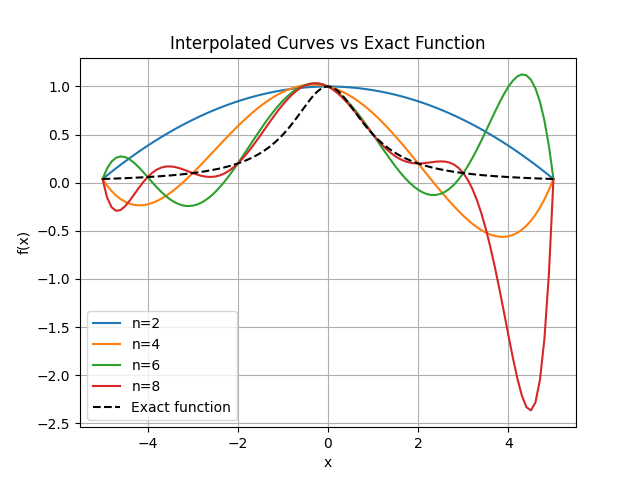
\includegraphics[width=\textwidth]{Report_figure/figure_B.png}
        \captionof{figure}{The graph obtained from the fitting in question B}
    \end{minipage}
    \hfill
    \begin{minipage}{0.45\textwidth}
        \centering
        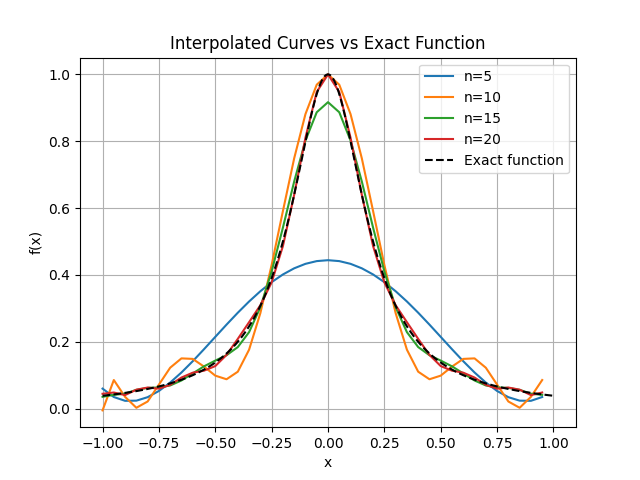
\includegraphics[width=\textwidth]{Report_figure/figure_C.png}
        \captionof{figure}{The graph obtained from the fitting in question C}
    \end{minipage}


\section*{D}

For the first question, directly invoke the Hermite interpolation method. \\
For the second question, a graph can be used for observation, but for simplicity, consider discretizing \( t \) with small step sizes. 
When the overspeed condition is met, output the corresponding time. The result is equivalent to fitting and observing through a graph.

\section*{E}

For question b, use the interpolation polynomial to estimate the daily weight for the next 15 days. 
If the weight \( \leq 0 \), it is considered as death, and the day of death should be output. 
Based on the output results, it is confirmed that neither of the two samples will die.
\begin{figure}[!h]
    \centering
    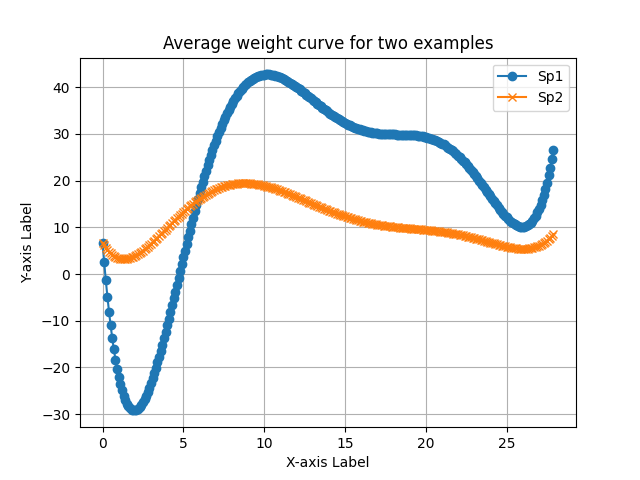
\includegraphics[width=0.5\linewidth]{Report_figure/figure_E.png}
    \caption{The weight curve obtained using Newton interpolation shows the changes over time.}
\end{figure}

\section*{F}

For this question, Algorithm 2.74 can be directly applied. However, one important point to note is the selection of points on the curve. 
Initially, points were selected only in the first and second quadrants, resulting in the fitting only approximating the upper portion of the curve. 
After identifying the cause, the point selection was corrected, leading to an approximation of the complete closed curve.
It can be noted that as the number of points increases, the curve fitting improves progressively.
    
    \begin{minipage}{0.45\textwidth}
        \centering
        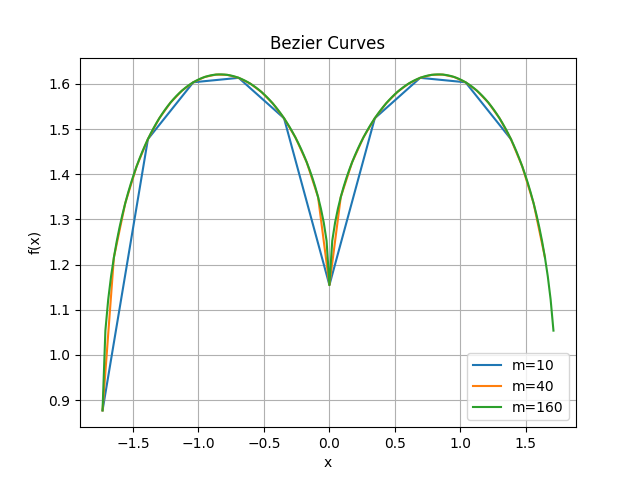
\includegraphics[width=\textwidth]{Report_figure/figure_F_incorrect.png}
        \captionof{figure}{Incorrect curve fitting}
    \end{minipage}
    \hfill
    \begin{minipage}{0.45\textwidth}
        \centering
        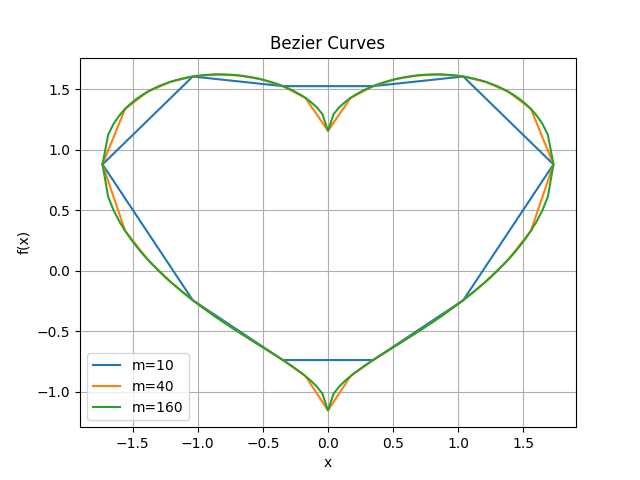
\includegraphics[width=\textwidth]{Report_figure/figure_F.png}
        \captionof{figure}{Complete bezier curves}
    \end{minipage}




% ===============================================
\subsection*{ \center{\normalsize {Acknowledgement}} }
\printbibliography

\end{document}